\begin{frame}{F5 load balancer exploit}
\begin{itemize}
\item c. 2021 F5 Big-IP load balancers shown to have stack buffer overflow
\item F5 didn't enable ASLR, write XOR execute
\item problem: stack address was randomized
\item so can't do stack smashing\ldots
\end{itemize}
\end{frame}

\begin{frame}[plain]{}
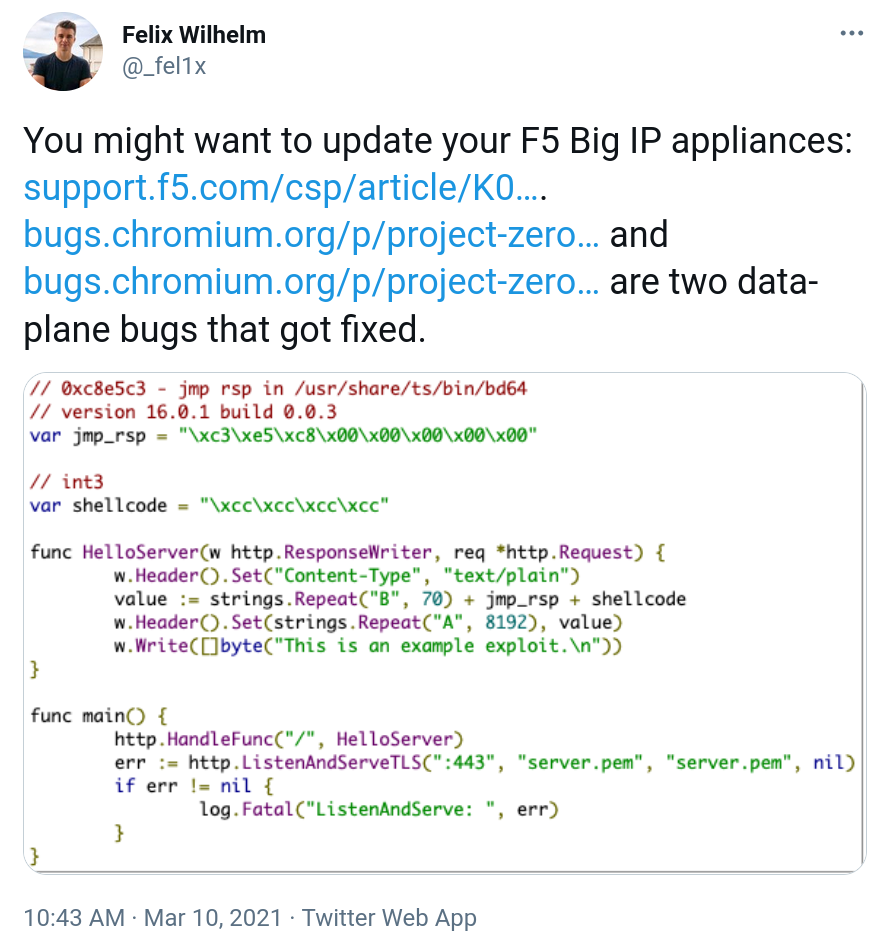
\includegraphics[height=0.95\textheight]{../rop/f5-poc-twitter}
\end{frame}

\begin{frame}[fragile,label=jmpRsp]{jmp *\%rsp}
    \begin{itemize}
    \item there was a \texttt{jmp *\%rsp} instruction at fixed address
    \vspace{.5cm}
    \item was that really lucky?
    \item let's try examining, say, \texttt{/bin/bash} (shell) on my desktop\ldots
    \end{itemize}
\begin{lstlisting}[language=,style=smaller]
   949bf:       8b 15 ff e4 08 00       mov    0x8e4ff(%rip),%edx
\end{lstlisting}
    \begin{itemize}
        \item machine code for \texttt{jmp *\%rsp}: \texttt{ff e4}
        \item \ldots appears in middle of mov instruction!
    \end{itemize}
\end{frame}

